




\documentclass{beamer}





\usepackage{pgf}%,pgfarrows,pgfnodes,pgfautomata,pgfheaps,pgfshade}
\usepackage{amsmath,amssymb}
%\usepackage[utf8]{inputenc}
\usepackage{colortbl}
%\usepackage{ngerman}
\usepackage{graphicx}
%\usepackage{here}
\usepackage{url}
\usepackage{pstricks}
%\usepackage{fancyvrb}
\usepackage{xspace}
\usepackage{multirow}
\usepackage{eurosym}
\usepackage{beamerthemeshadow}
\beamersetuncovermixins{\opaqueness<1>{25}}{\opaqueness<2->{15}}

\usepackage[latin1]{inputenc}
\usepackage[T1]{fontenc}  
\usepackage[francais]{babel}

% general
%\newcommand{\quota}[1]{``#1''}
\newcommand{\quota}[1]{\glqq{}#1\grqq{}}
\definecolor{lightred}{rgb}{1,0.3,0.3}
\definecolor{lightgreen}{rgb}{0.3,1,0.3}
\definecolor{lightblue}{rgb}{0.5,0.5,1}
\definecolor{darkred}{rgb}{0.7,0,0}
%\newcommand{\redmathbox}[1]{\colorbox{lightred}{\ensuremath{#1}}}
%\newcommand{\greenmathbox}[1]{\colorbox{lightgreen}{\ensuremath{#1}}}
%\newcommand{\pseudomathbox}[1]{\setlength{\fboxrule}{0pt}\fbox{\ensuremath{#1}}\setlength{\fboxrule}{1pt}}

\newcommand{\redbox}[1]{\colorbox{lightred}{#1}}
\newcommand{\greenbox}[1]{\colorbox{lightgreen}{#1}}
\newcommand{\bluebox}[1]{\colorbox{lightblue}{#1}}
\newcommand{\yellowbox}[1]{\colorbox{yellow}{#1}}

\setlength{\fboxrule}{1pt}


%% Das Layout
\setbeamertemplate{footline} %% Eine Fußzeile für die Slide-Nummern
{%
  \hbox{%
  \begin{beamercolorbox}[wd=.25\paperwidth,ht=2.25ex,dp=1ex,center]{author in head/foot}%
    \usebeamerfont{title in head/foot}\insertshortauthor
  \end{beamercolorbox}%
  \begin{beamercolorbox}[wd=.5\paperwidth,ht=2.25ex,dp=1ex,center]{title in head/foot}%
    \usebeamerfont{title in head/foot}\insertshorttitle
  \end{beamercolorbox}%
  \begin{beamercolorbox}[wd=.25\paperwidth,ht=2.25ex,dp=1ex,center]{date inhead/foot}%
    \insertframenumber{} / \inserttotalframenumber
    \hspace*{2ex}
  \end{beamercolorbox}}%
  \vskip0pt%
}
%\usefonttheme[onlysmall]{structurebold} %% Schriftlayout
\setbeamercovered{transparent}
%\setbeamertemplate{navigation symbols}{} %% Abschalten der Navigation

\title{Finding Genes With HMMs}
\subtitle{INF 582 - Datamining}
\author{Till Rohrmann, Damien Arnol}
%\institute{SciEngines GmbH}
\date{March 2013}

% Gliederung bei Sektionsanfang
 \AtBeginSection[]
 {
   %\logo{}
   \begin{frame}
     %\frametitle{Übersicht}
     \tableofcontents[current,hideothersubsections,subsectionstyle=show/shaded/hide,subsubsectionstyle=show/shaded/hide]
   \end{frame}%\note{}
 }

% Gliederung bei Subsektionsanfang
  \AtBeginSubsection[]
  {
    \logo{}
    \begin{frame}
      %\frametitle{Übersicht}
      \tableofcontents[current,currentsubsection,subsectionstyle=show/shaded/hide,subsectionstyle=show/shaded/hide,subsubsectionstyle=show/shaded/hide]
    \end{frame}\note{}
  }

%% Gliederung bei Subsubsektionsanfang
%  \AtBeginSubsubsection[]
%  {
%    \logo{}
%    \begin{frame}
%      %\frametitle{Übersicht}
%      \tableofcontents[current,currentsubsection,subsectionstyle=show/shaded/hide,subsectionstyle=show/shaded/hide,subsubsectionstyle=show/shaded/hide]
%    \end{frame}\note{}
%  }

% ----------------------------------------------- BEGINNING OF THE DOCUMENT ----------------------------------------------- %
%% Das Dokument
\begin{document}

\frame{
	\titlepage
}

%\begin{frame}
%\frametitle{Apper\c cu g\'en\'eral du projet}
%\textbf{Objectif :}
%\begin{itemize}
%	\item Mod\'eliser la langue fran\c caise par un processus de Markov d'ordre $n$
%	\item Calculer l'entropie par lettre de cette source markovienne pour diff\'erents ordres
%	\item Impl\'ementer un g\'en\'erateur al\'eatoire de texte
%\end{itemize}
%
%\textbf{D\'emarche : 3 phases}
%\begin{itemize}
%	\item Apprentissage : d\'etermination des probabilit\'es d'\'emission conditionnelles de cette source
%	\item Calcul de l'entropie par lettre
%	\item Restitution
%\end{itemize}
%
%\textbf{R\'esultats}
%\begin{itemize}
%	\item Un programme fonctionnant correctement pour tout ordre
%\end{itemize}
%
%\end{frame}


\frame{
  \frametitle{Outline}
  \tableofcontents[hideallsubsections]
}


\section{HMMs and implementation}
\subsection{Description of the probabilistic model}

\begin{frame}
\frametitle{Description of the probabilistic model}
\begin{columns}

		\column{0.50\textwidth}
		\begin{figure}[h]
			\centering
			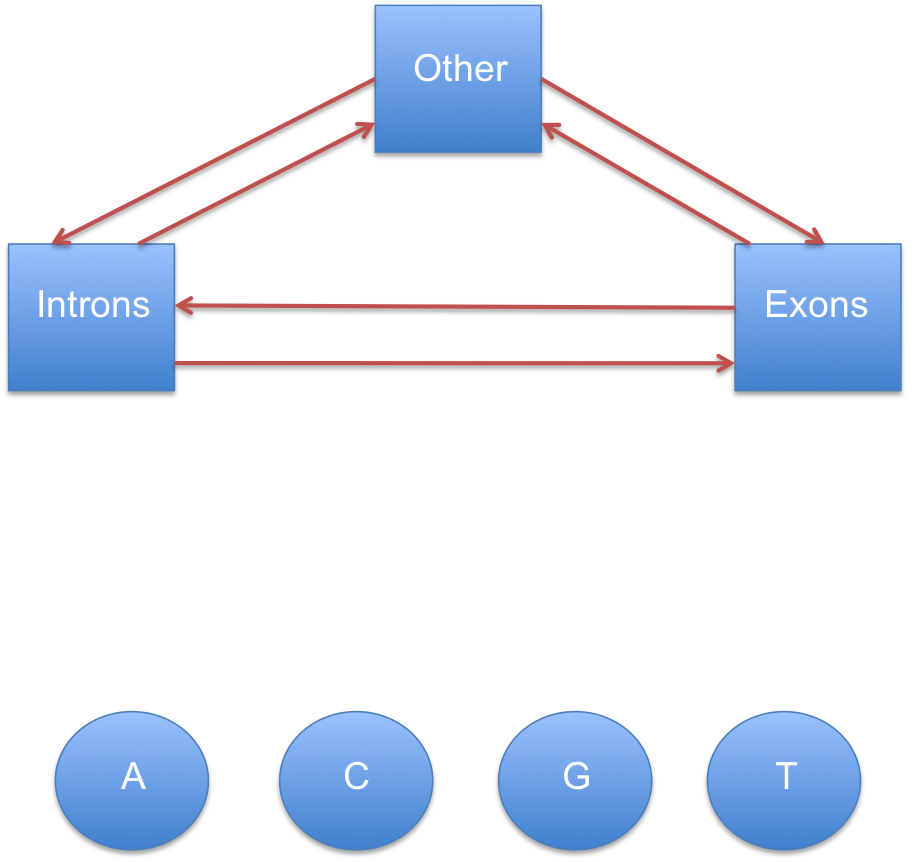
\includegraphics[width=1.0\textwidth]{../picturesforthepresentation/HMM1.png}<1>
			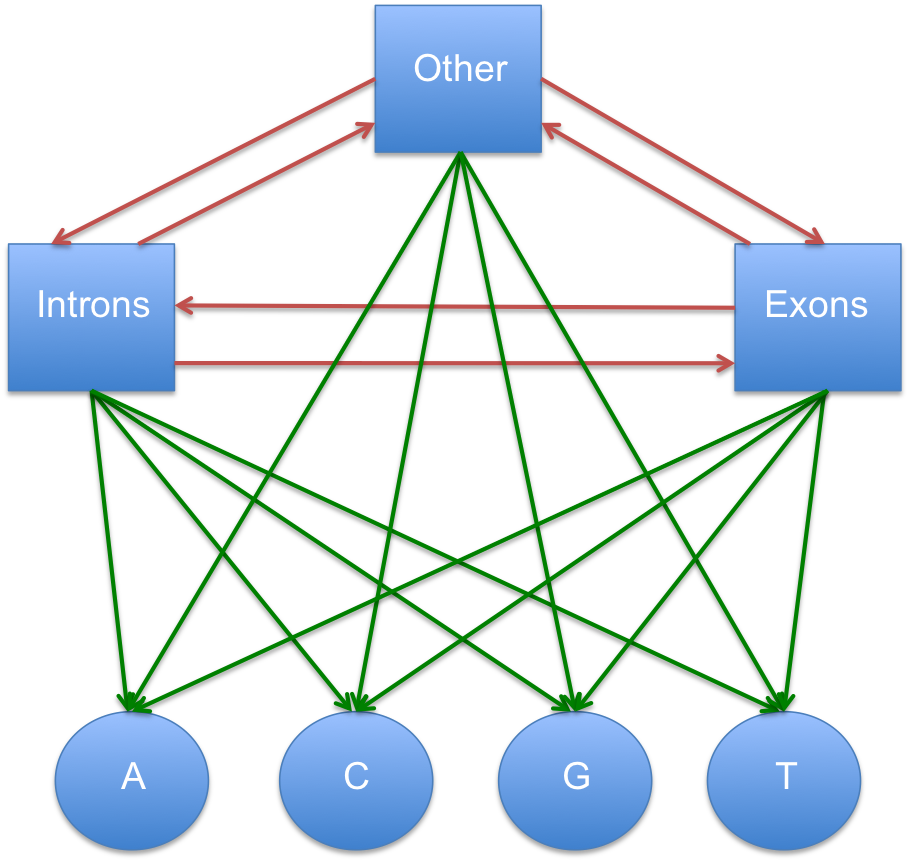
\includegraphics[width=1.0\textwidth]{../picturesforthepresentation/HMM2.png}<2>		
		\end{figure}
		
		\column{0.50\textwidth}
		\begin{block}{Transition Probabilities}<1>
		%\vspace{0.1cm}
			from state i to state j: $T_{ij}$\\
		
		\end{block}
		\vspace{0.3cm}
		\begin{block}{Emission Probabilities}<2>
		%\vspace{0.1cm}
			Emission of A being in state i: $E(A|i)$
		\end{block}
\end{columns}
\end{frame}

\subsection{Decoding a sequence of emitted states}

\begin{frame}
\frametitle{The viterbi algorithm}

		\begin{figure}[h]
			\centering
			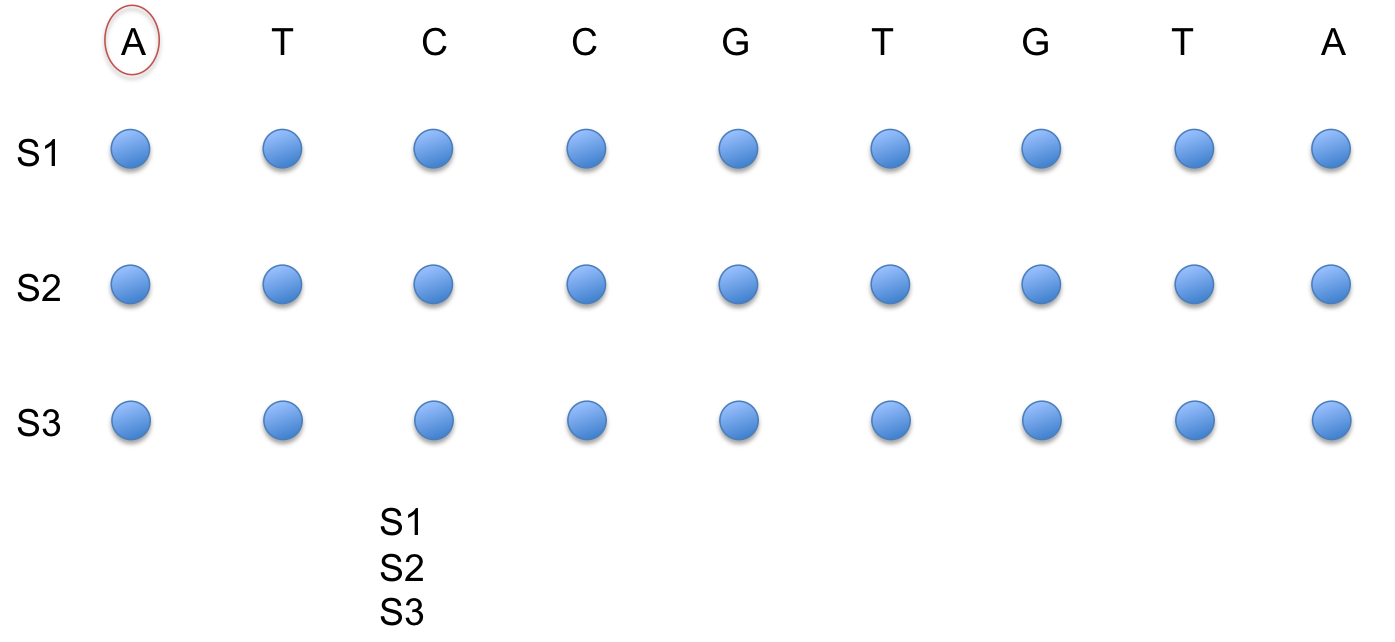
\includegraphics[width=1.0\textwidth]{../picturesforthepresentation/Viterbi1.png}<1>
			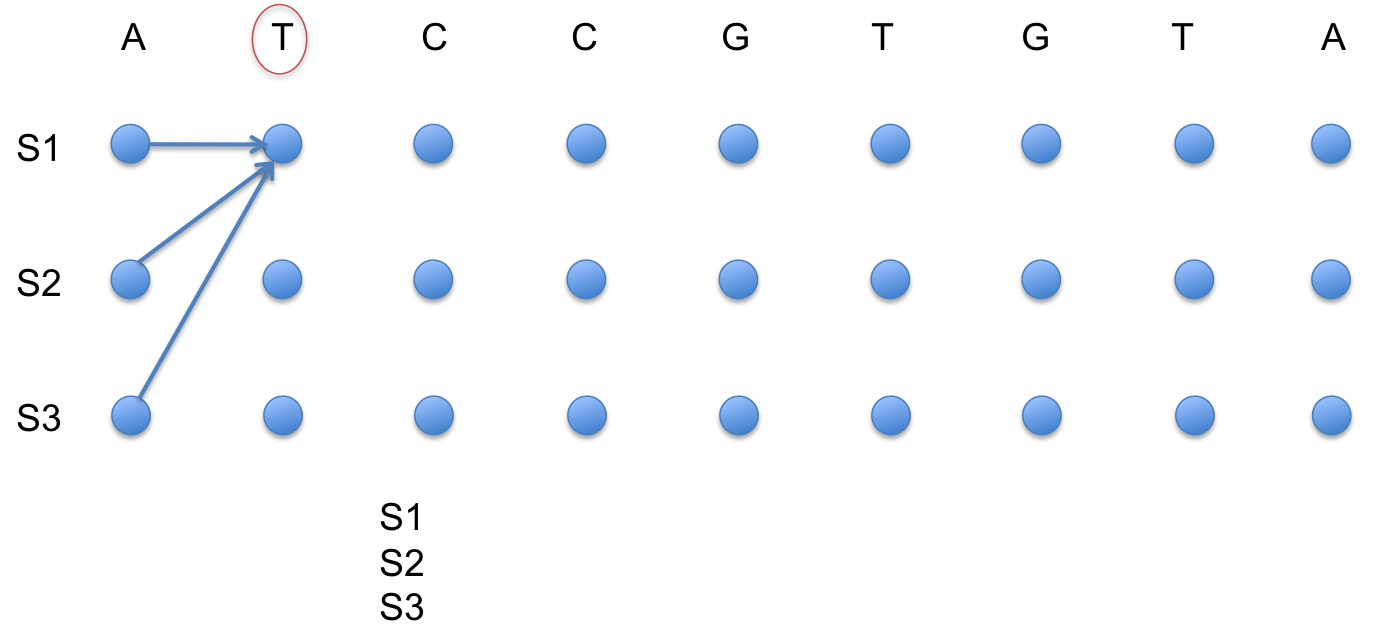
\includegraphics[width=1.0\textwidth]{../picturesforthepresentation/Viterbi2.png}<2>
			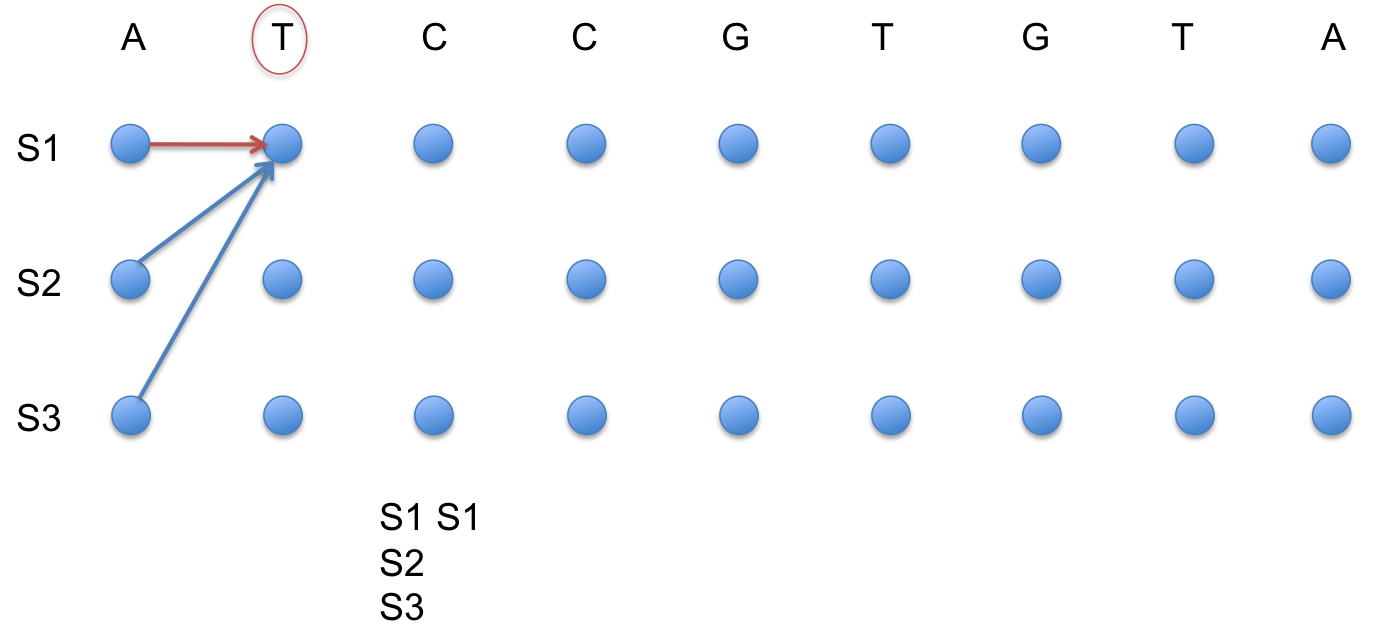
\includegraphics[width=1.0\textwidth]{../picturesforthepresentation/Viterbi3.png}<3>
			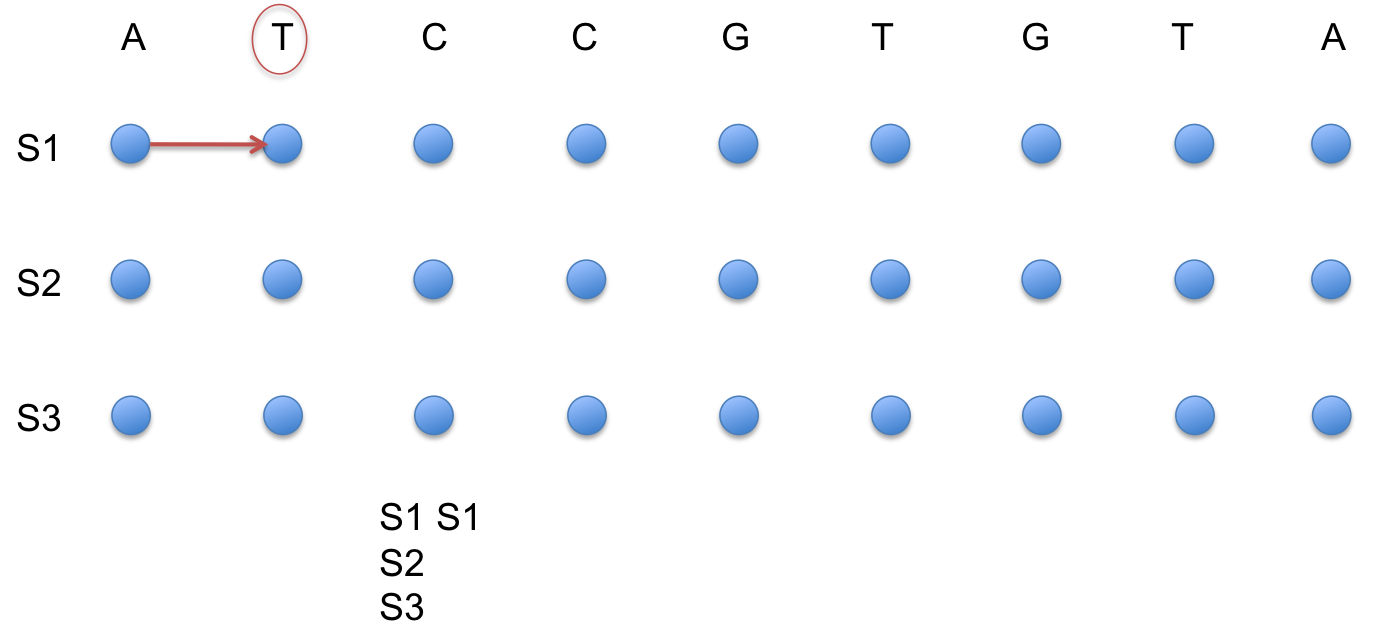
\includegraphics[width=1.0\textwidth]{../picturesforthepresentation/Viterbi4.png}<4>
			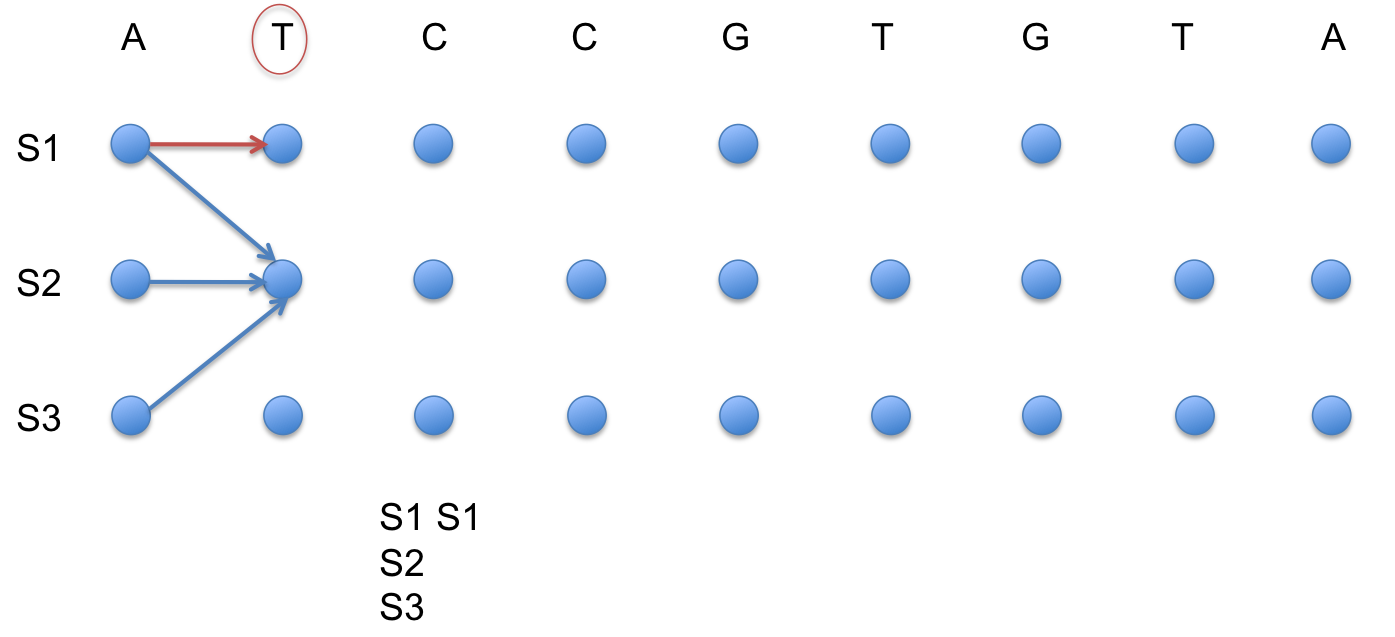
\includegraphics[width=1.0\textwidth]{../picturesforthepresentation/Viterbi5.png}<5>
			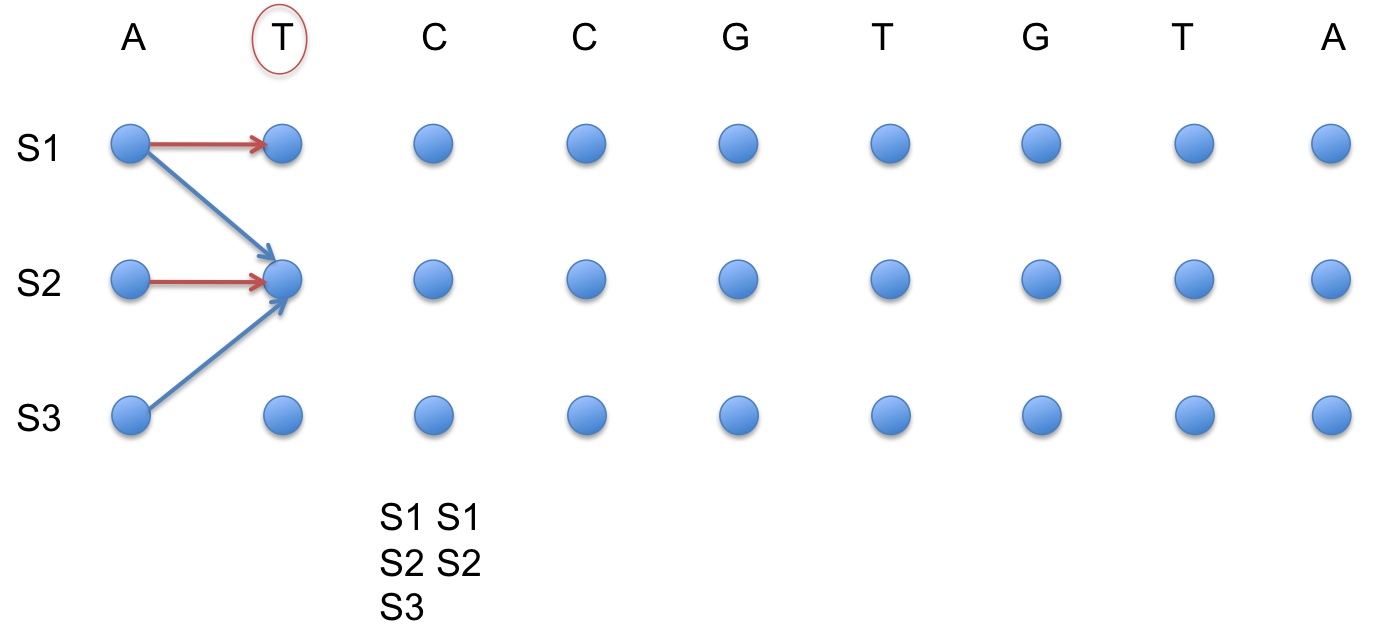
\includegraphics[width=1.0\textwidth]{../picturesforthepresentation/Viterbi6.png}<6>
			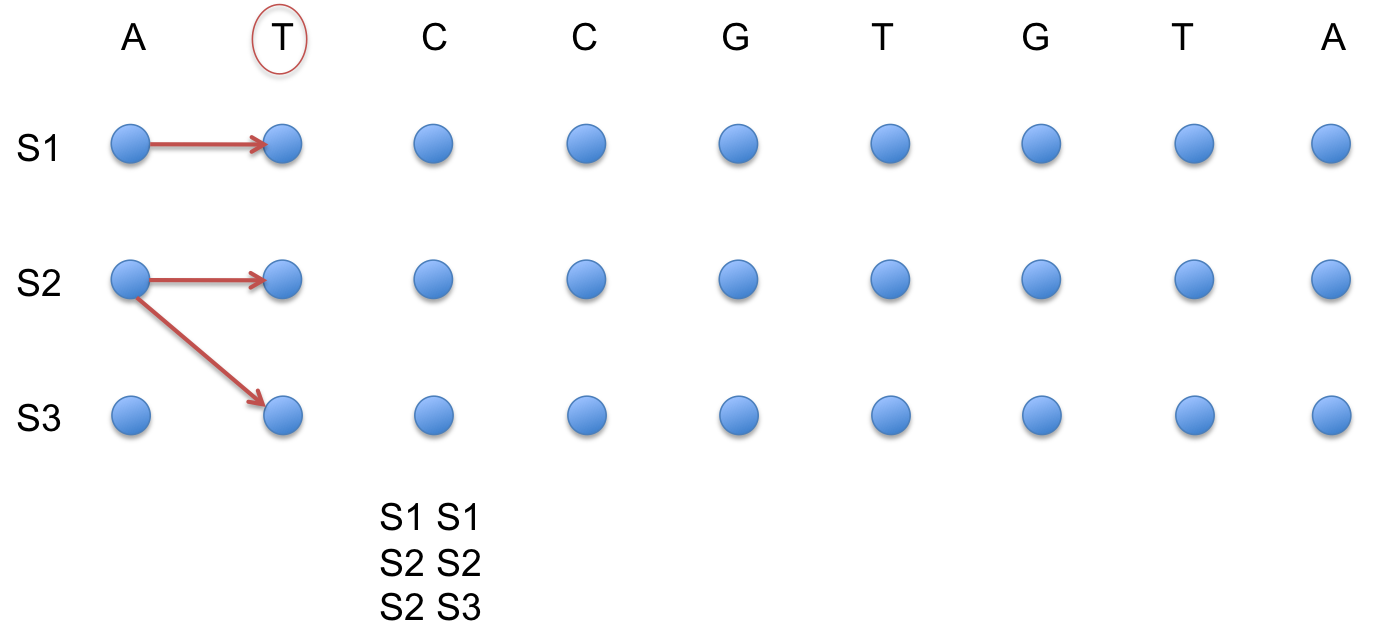
\includegraphics[width=1.0\textwidth]{../picturesforthepresentation/Viterbi7.png}<7>
			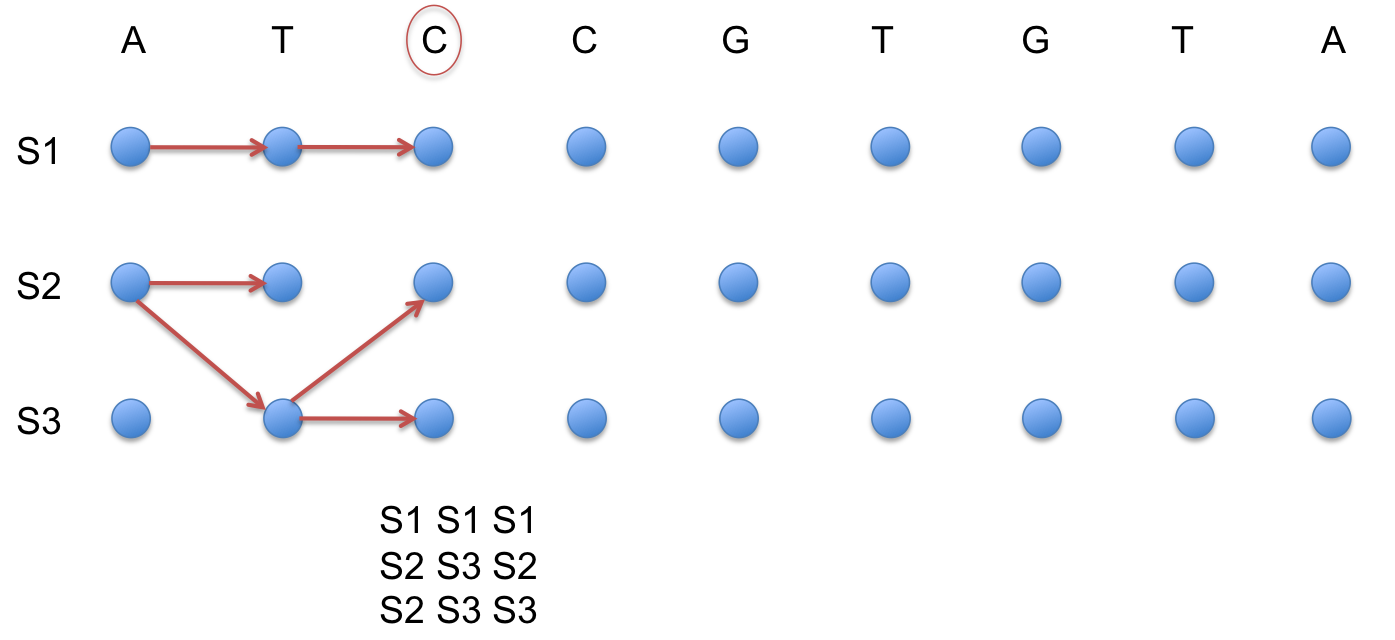
\includegraphics[width=1.0\textwidth]{../picturesforthepresentation/Viterbi8.png}<8>
			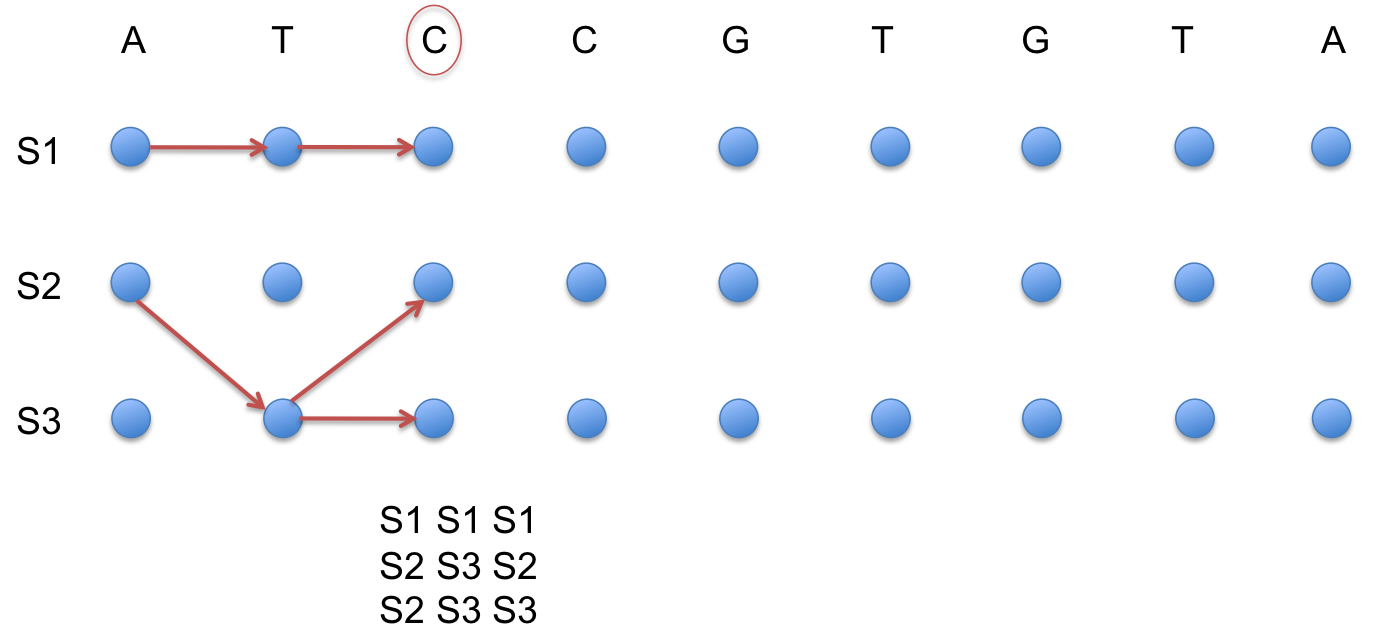
\includegraphics[width=1.0\textwidth]{../picturesforthepresentation/Viterbi9.png}<9>
			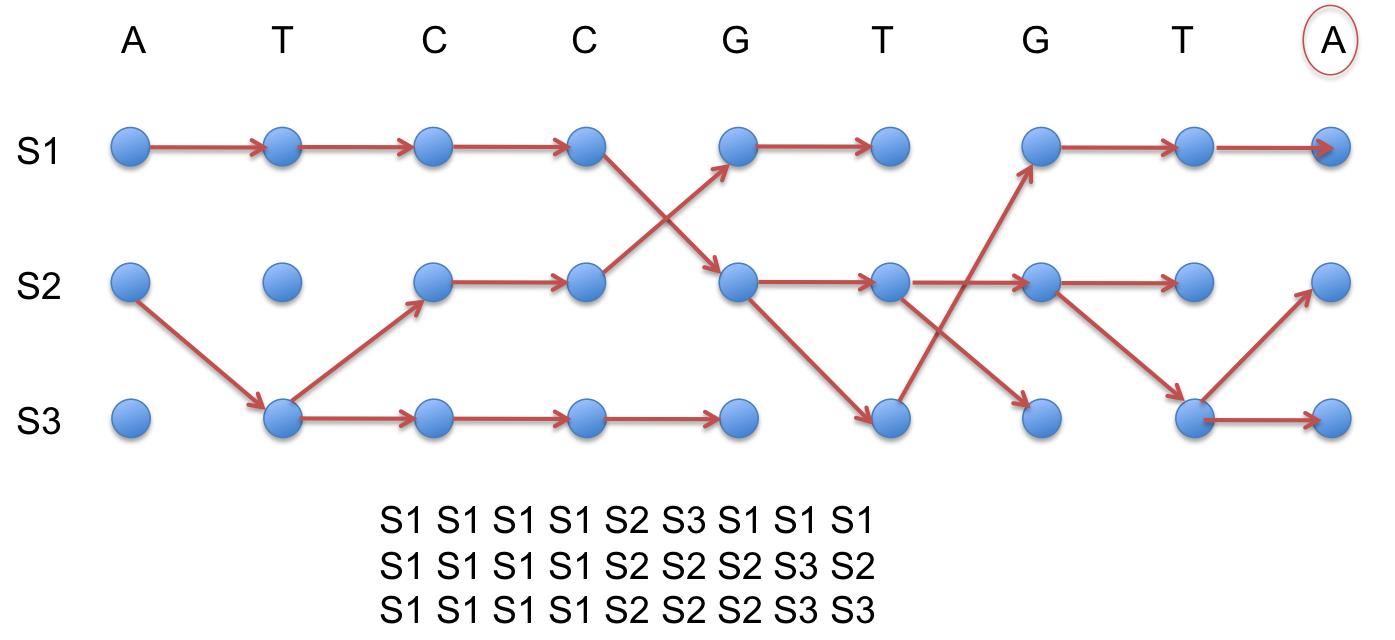
\includegraphics[width=1.0\textwidth]{../picturesforthepresentation/Viterbi10.png}<10>
			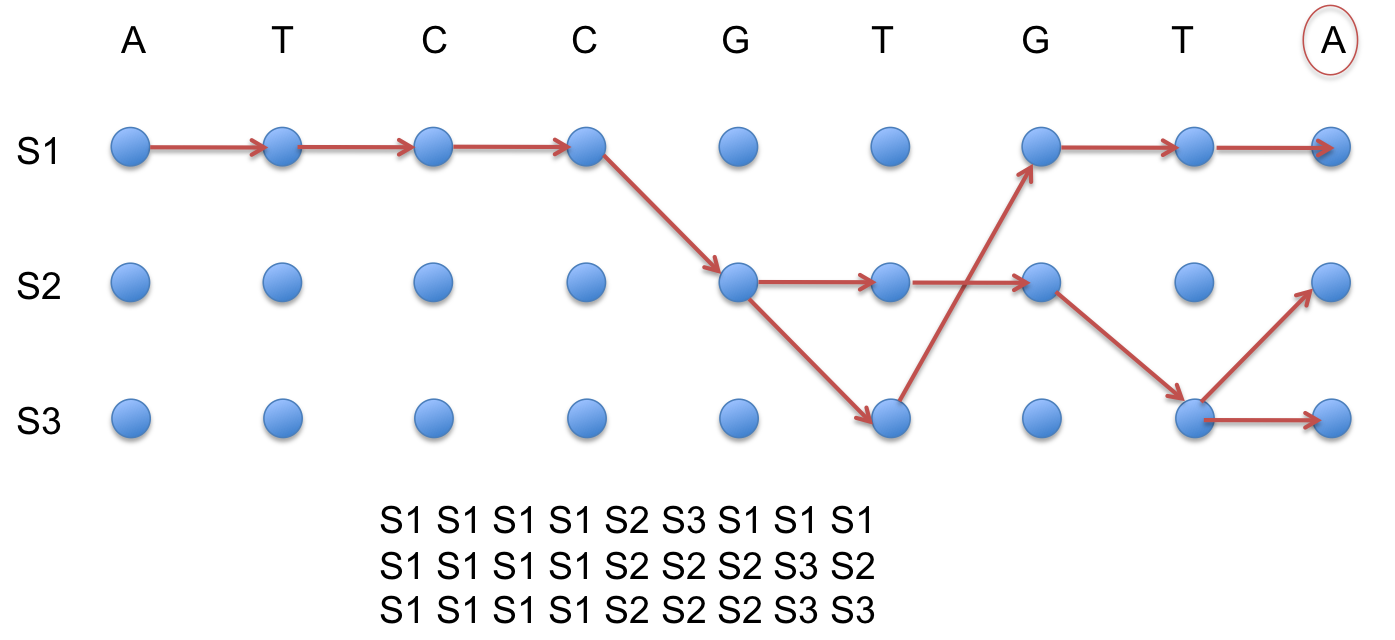
\includegraphics[width=1.0\textwidth]{../picturesforthepresentation/Viterbi11.png}<11>
			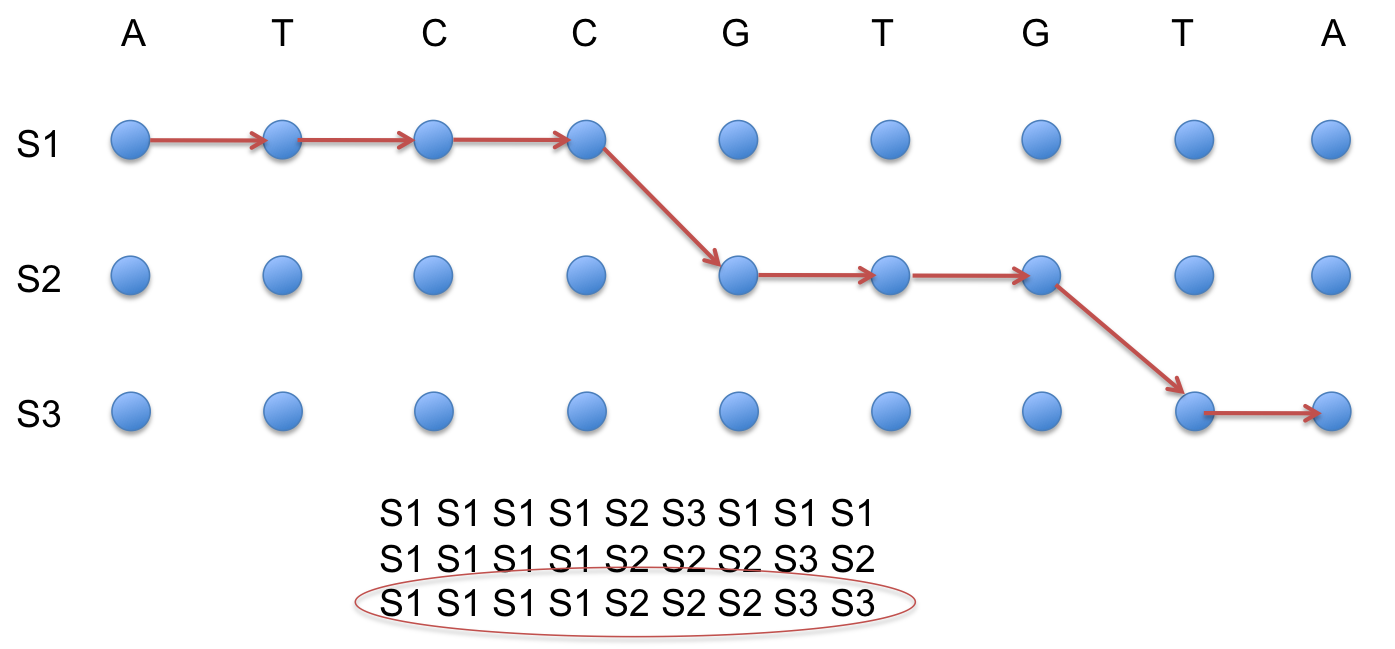
\includegraphics[width=1.0\textwidth]{../picturesforthepresentation/Viterbi12.png}<12>			
		\end{figure}

\end{frame}


\begin{frame}
\frametitle{Formal writing}

\begin{block}{Additional Notations}
$(y_1...y_n)$ : sequence of bases to decode\\
$S$ : space of the possible states\\
$\pi_{k}$ : Probability of beginning in state k\\
$V_{t,k}$ : probability of the best track ending in state k at step t
\end{block}

\begin{block}{Initialization}
\begin{equation*}
V_{1,k} = E(y_1|k)\times\pi_{k}
\end{equation*}
\end{block}

\begin{block}{Recursion}
\begin{equation*}
\forall k\ V_{t,k} = E(y_t|k)\times\max_{x \in S}\big(T_{xk}\times V_{T,x}\big)
\end{equation*}
\begin{equation*}
x_{T} = argmax_{x \in S}\big(V_{T,x}\big)
\end{equation*}
\end{block}

\end{frame}

\subsection{Learning process}

\begin{frame}
\frametitle{Principle}
\begin{figure}[h]
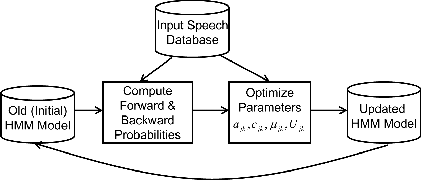
\includegraphics[width=1.0\textwidth]{../picturesforthepresentation/baumwelch.png}
\end{figure}

\end{frame}

\section{Biological applications}
\subsection{Relevance of the previous simple model}

\begin{frame}
\frametitle{Exons and introns show different statistical pattern}
\begin{itemize}
	\item G-C Content is higher in exons
	\item differences in the frequency of codon usage
	\item periodicity of certain bases due to codon usage
\end{itemize}
		
	\vspace{0.5cm}
	
	\pause\begin{center}
		\textbf{We need a three-stage model }
	\end{center}
\end{frame}

\subsection{How to inject more biological information}
\begin{frame}
\frametitle{Weaknesses of the intron-exon model}
	\begin{itemize}
		\item No splicing sites recognition 
		\item How to take into account a STOP codon ? 
		\item Promoters and START codons ? 
		\item Poly-A sites ?
	\end{itemize}
	
	\vspace{0.5cm}
	
	\pause\begin{center}
		\textbf{We should define more states without allowing all transitions}
	\end{center}
	
\end{frame}

\begin{frame}
\frametitle{The implementation we chose}
	\begin{figure}
	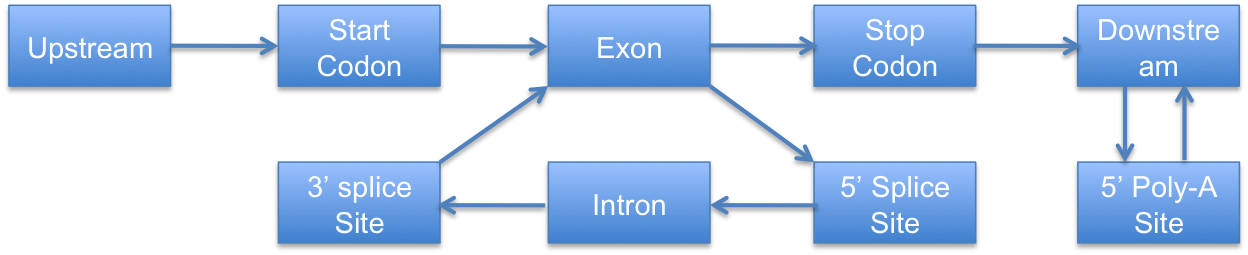
\includegraphics[width=1.0\textwidth]{../picturesforthepresentation/combinedHMM.png}
	\end{figure}
	
	\begin{itemize}
		\item 5' Splice sites are 9-stage models
		\item 3' Splice sites are 5-stage models
		\item Poly-A sites are 6-stage models 
	\end{itemize}
	
	\pause\begin{center}
		\textbf{the different several-stages models work like autonomous HMMs}
	\end{center}
	
\end{frame}




\end{document}
